\chapter{Wyniki eksperymentalne i walidacja modeli}
\label{ch:wyniki}

\section{Metodyka przeprowadzonych badań i model w programie Simulink}
\label{sec:metodyka}

W celu dokonania rzetelnej oceny dokładności modeli, badania przeprowadzono
w układzie zamkniętym sprzężenia zwrotnego. Zastosowane w badaniach nastawy
regulatora PID zostały wyznaczone empirycznie podczas wielokrotnych prób
optymalnego dostrojenia regulatora bezpośrednio na rzeczywistym stanowisku
laboratoryjnym.

Badania polegały na rejestracji odpowiedzi układu na skokową zmianę
wartości zadanej (setpointu). Wybrano dwa reprezentatywne stany wymuszeń,
które pozwalają ocenić zachowanie kulki w obu kierunkach ruchu:
\begin{enumerate}
    \item \textbf{Skok wartości zadanej w górę (plik \texttt{proba1.csv})}:
    krok ze 124~mm do 172~mm (amplituda $+48$~mm).
    \item \textbf{Skok wartości zadanej w dół (plik \texttt{proba2.csv})}:
    krok ze 125~mm do 40~mm (amplituda $-85$~mm).
\end{enumerate}

Okres próbkowania pętli regulacji wynosił $T_s = 0.032$~s. Podczas wszystkich
prób rzeczywistych regulator PID zaimplementowany na mikrokontrolerze
posiadał stałe nastawy zdefiniowane jako: $K_{p\text{\_STM}} = 0.26$,
$K_{i\text{\_STM}} = 0.0064$ oraz $K_{d\text{\_STM}} = 4.4$.

Zarejestrowane przebiegi czasowe odpowiedzi rzeczywistego obiektu (zarówno
pozycji kulki, jak i sygnału sterującego) dla obu prób przedstawiono na
rysunkach~\ref{fig:proba1_raw} oraz~\ref{fig:proba2_raw}.

\begin{figure}[H]
    \centering
    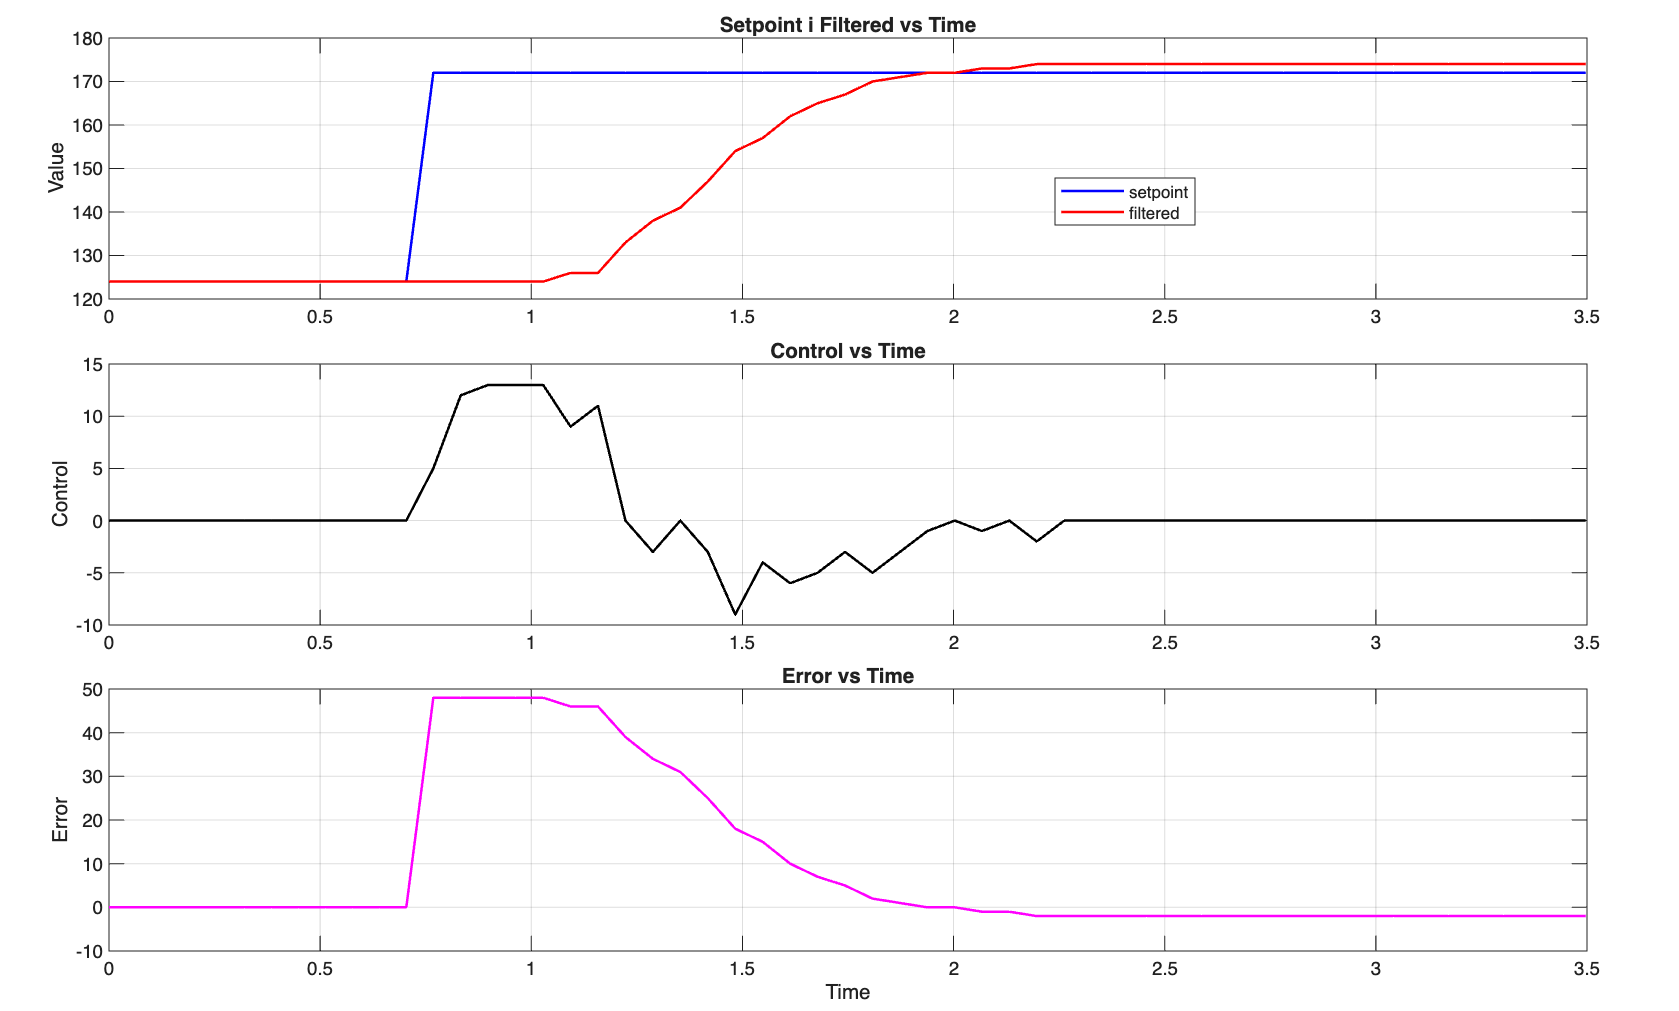
\includegraphics[width=\linewidth]{4-wyniki-eksperymentalne/img/proba1_plots.png}
    \caption{Przebiegi czasowe pozycji kulki oraz sygnału sterującego
    dla rzeczywistego obiektu — skok w górę (amplituda +48 mm, plik \texttt{proba1})}
    \label{fig:proba1_raw}
\end{figure}

\begin{figure}[H]
    \centering
    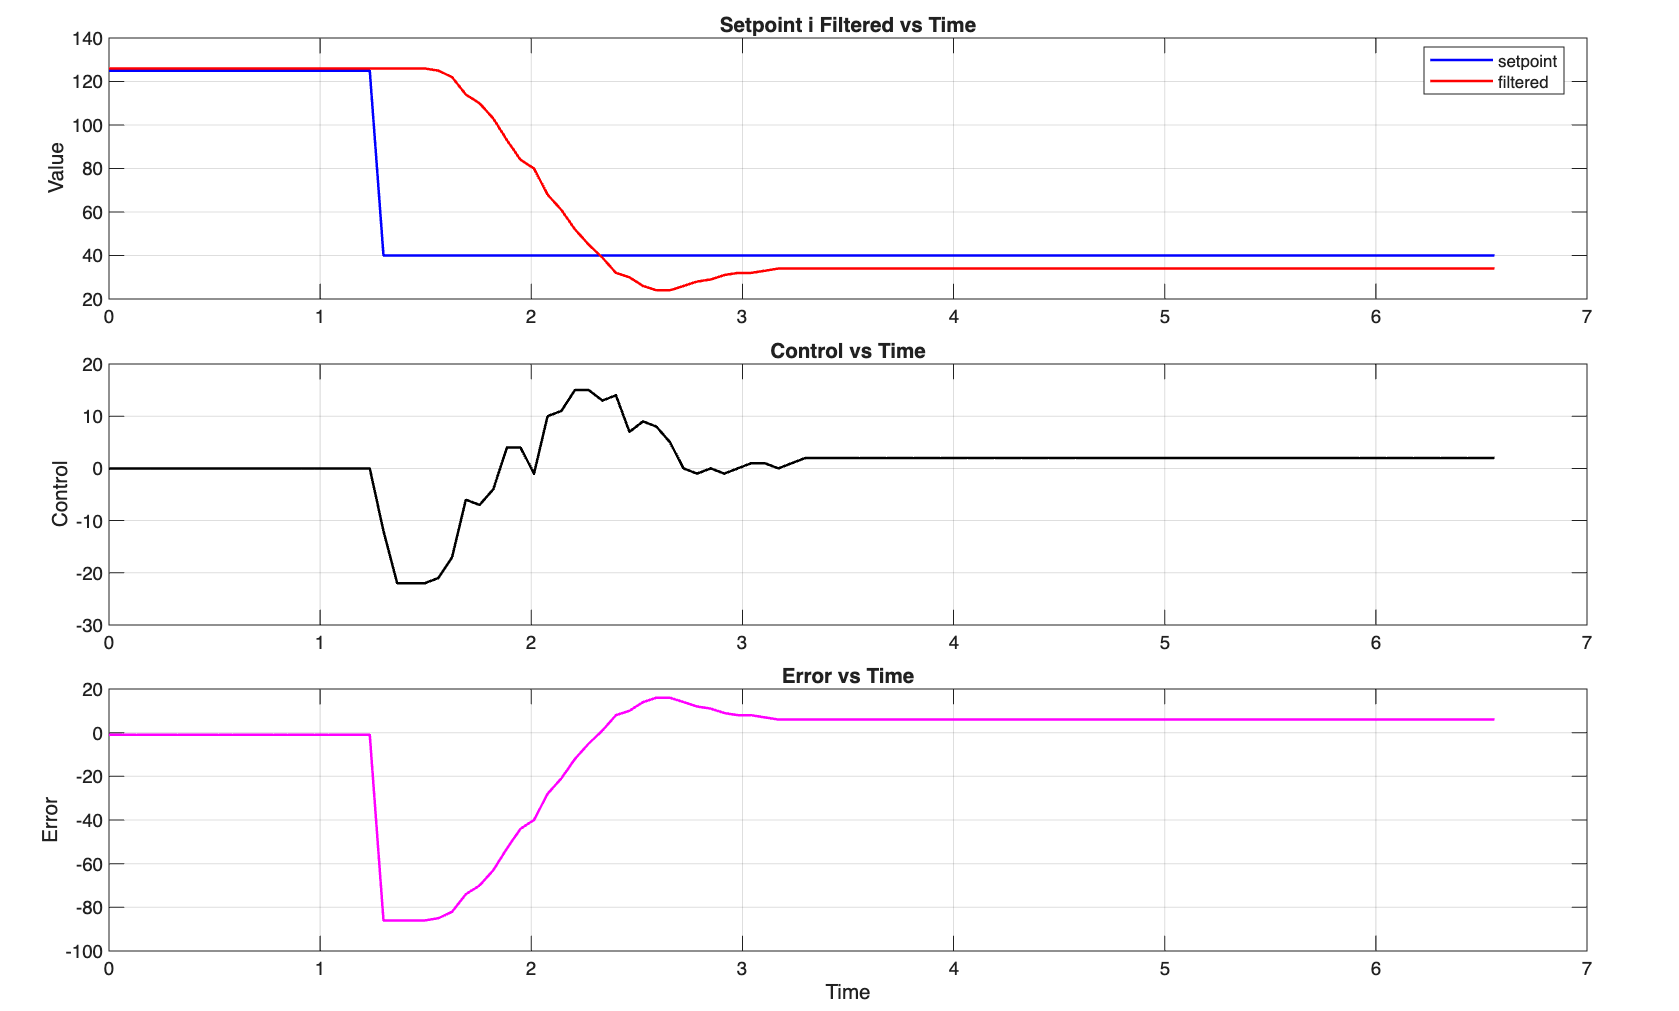
\includegraphics[width=\linewidth]{4-wyniki-eksperymentalne/img/proba2_plots.png}
    \caption{Przebiegi czasowe pozycji kulki oraz sygnału sterującego
    dla rzeczywistego obiektu — skok w dół (amplituda -85 mm, plik \texttt{proba2})}
    \label{fig:proba2_raw}
\end{figure}

\subsection{Struktura modelu symulacyjnego w programie Simulink}
Model symulacyjny w programie Simulink został zbudowany od podstaw w celu
rzetelnego odwzorowania rzeczywistego stanowiska. Oprócz zamkniętej pętli
sterowania z modelami obiektów (teoretycznym i doświadczalnym) oraz blokiem
regulatora, w schemacie zaimplementowano dwa tory obliczeniowe do wyznaczania
wskaźników jakości regulacji w czasie rzeczywistym symulacji:
\begin{itemize}
    \item \textbf{Wskaźnik całkowy ITAE}: zaimplementowany poprzez pobranie
    bezwzględnej wartości uchybu (blok \texttt{Abs}), pomnożenie jej przez czas
    symulacji (blok \texttt{Clock}) za pomocą bloku mnożącego (\texttt{Product})
    oraz skierowanie wyniku na blok całkujący (\texttt{Integrator}). Wyjście
    integratora podłączono do bloku wyświetlacza (\texttt{ITAE}), z którego
    bezpośrednio odczytywana jest wartość końcowa wskaźnika:
    \begin{equation}
        \text{ITAE} = \int_{0}^{T} t \cdot |e(t)| \, dt
    \end{equation}
    \item \textbf{Wskaźnik energii (kosztu) sterowania}: zaimplementowany
    poprzez pobranie nasyconego sygnału sterującego $u(t)$ (odchylenia belki od
    poziomu), podniesienie go do kwadratu (blok \texttt{Math Function} w trybie
    \texttt{square}) oraz zintegrowanie za pomocą bloku całkującego
    (\texttt{Integrator}). Wartość kosztu odczytywana jest bezpośrednio z bloku
    wyświetlacza (\texttt{Koszt sterowania}):
    \begin{equation}
        J_u = \int_{0}^{T} u^2(t) \, dt
    \end{equation}
\end{itemize}
Dzięki temu model symulacyjny automatycznie wyznacza wskaźniki jakości podczas
każdego przebiegu, co eliminuje konieczność ręcznego całkowania przebiegów
wyjściowych.

\begin{figure}[H]
    \centering
    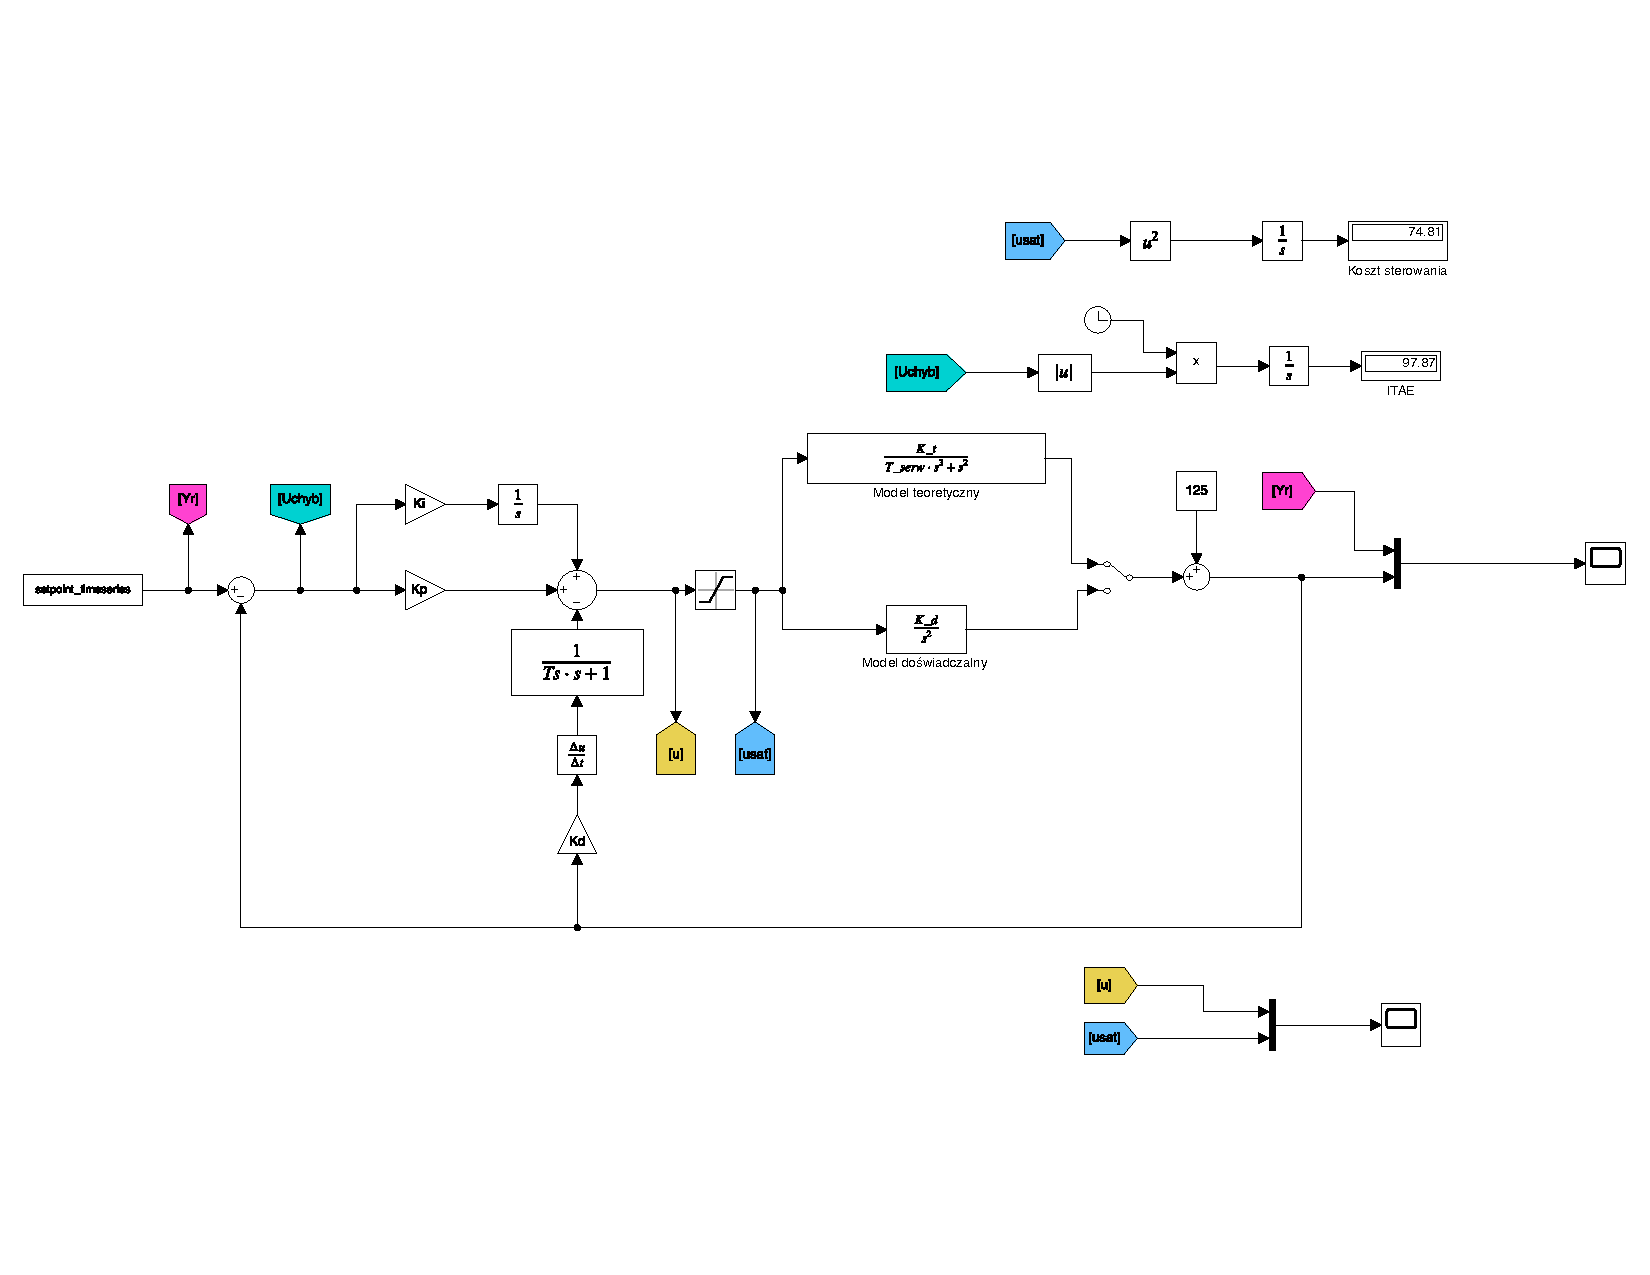
\includegraphics[width=\linewidth]{4-wyniki-eksperymentalne/img/ballonbeam_matlab1.pdf}
    \caption{Schemat blokowy układu regulacji w programie Simulink wraz
    z torami obliczania wskaźników jakości ITAE oraz kosztu sterowania}
    \label{fig:simulink_model}
\end{figure}

\subsection{Przeliczenie nastaw regulatora (STM32 $\rightarrow$ Simulink)}
Wygodne przenoszenie parametrów regulatora z mikrokontrolera do ciągłego
modelu w programie Simulink wymagało uwzględnienia specyfiki dyskretnej
implementacji kodu w C. W strukturze kodu sterującego na STM32, w celu
optymalizacji obliczeniowej (uniknięcie powolnych operacji dzielenia
zmiennoprzecinkowego w przerwaniu), pominięto okres próbkowania $T_s$
w równaniach członu całkującego i różniczkującego.

Dyskretny algorytm sterowania zaimplementowany na STM32 opisują następujące
zależności :
\begin{equation}
    P_k = K_{p\text{\_STM}} \cdot e_k
\end{equation}
\begin{equation}
    I_k = K_{i\text{\_STM}} \cdot \sum_{j=1}^{k} e_j
\end{equation}
\begin{equation}
    D_k = K_{d\text{\_STM}} \cdot (y_{k-1} - y_k)
\end{equation}
gdzie $y_k$ oznacza przefiltrowaną pozycję kulki w kroku $k$
(różniczkowanie po pomiarze w celu eliminacji tzw. \textit{derivative kick}).

W ciągłym i równoległym modelu w programie Simulink, klasyczne równania
członów regulatora mają postać ciągłą:
\begin{equation}
    P(t) = K_{p\text{\_Sim}} \cdot e(t)
\end{equation}
\begin{equation}
    I(t) = K_{i\text{\_Sim}} \int_{0}^{t} e(\tau) \, d\tau \approx K_{i\text{\_Sim}} \cdot T_s \sum_{j=1}^{k} e_j
\end{equation}
\begin{equation}
    D(t) = -K_{d\text{\_Sim}} \frac{dy(t)}{dt} \approx -K_{d\text{\_Sim}} \frac{y_k - y_{k-1}}{T_s} = K_{d\text{\_Sim}} \frac{y_{k-1} - y_k}{T_s}
\end{equation}
Porównując dyskretne równania z kodu C mikrokontrolera z ich ciągłymi
przybliżeniami stosowanymi w Simulinku, wyznaczono dokładne zależności
skalujące nastawy:
\begin{itemize}
    \item \textbf{Człon proporcjonalny}: Jest tożsamy w obu środowiskach:
    \begin{equation}
        K_{p\text{\_Sim}} = K_{p\text{\_STM}} = 0.26
    \end{equation}
    \item \textbf{Człon całkujący}: W kodzie C brak mnożenia przez $T_s$,
    stąd w Simulinku (gdzie blok całki integruje po czasie ciągłym) wzmocnienie
    całki (blok \texttt{1/Ti}) musi zostać podzielone przez $T_s$:
    \begin{equation}
        K_{i\text{\_Sim}} = \frac{K_{i\text{\_STM}}}{T_s} = \frac{0.0064}{0.032} = 0.20
    \end{equation}
    \item \textbf{Człon różniczkujący}: W kodzie C brak dzielenia przez $T_s$
    przy wyznaczaniu różnicy próbek, stąd w Simulinku (gdzie blok
    różniczkujący dzieli przez $\Delta t$) wzmocnienie różniczki (blok
    \texttt{Td}) musi zostać pomnożone przez $T_s$:
    \begin{equation}
        K_{d\text{\_Sim}} = K_{d\text{\_STM}} \cdot T_s = 4.4 \cdot 0.032 = 0.1408
    \end{equation}
\end{itemize}

\section{Przebiegi czasowe i weryfikacja modeli}
\label{sec:przebiegi}

W celu weryfikacji porównano przebiegi czasowe pozycji kulki oraz sygnału
sterującego dla obiektu rzeczywistego, modelu teoretycznego:
\begin{equation}
    G_{\text{teor}}(s) = \frac{20.55}{s^2(0.095s + 1)}
\end{equation}
oraz modelu doświadczalnego:
\begin{equation}
    G_{\text{dosw}}(s) = \frac{11.93}{s^2(0.095s + 1)}
\end{equation}

Porównawcze przebiegi czasowe pozycji kulki oraz sygnałów sterujących dla obu
prób przedstawiono na rysunkach \ref{fig:proba1_pos_teor}--\ref{fig:proba1_u_dosw}
(dla skoku w górę) oraz na rysunkach \ref{fig:proba2_pos_teor}--\ref{fig:proba2_u_dosw}
(dla skoku w dół). 

\begin{figure}[H]
    \centering
    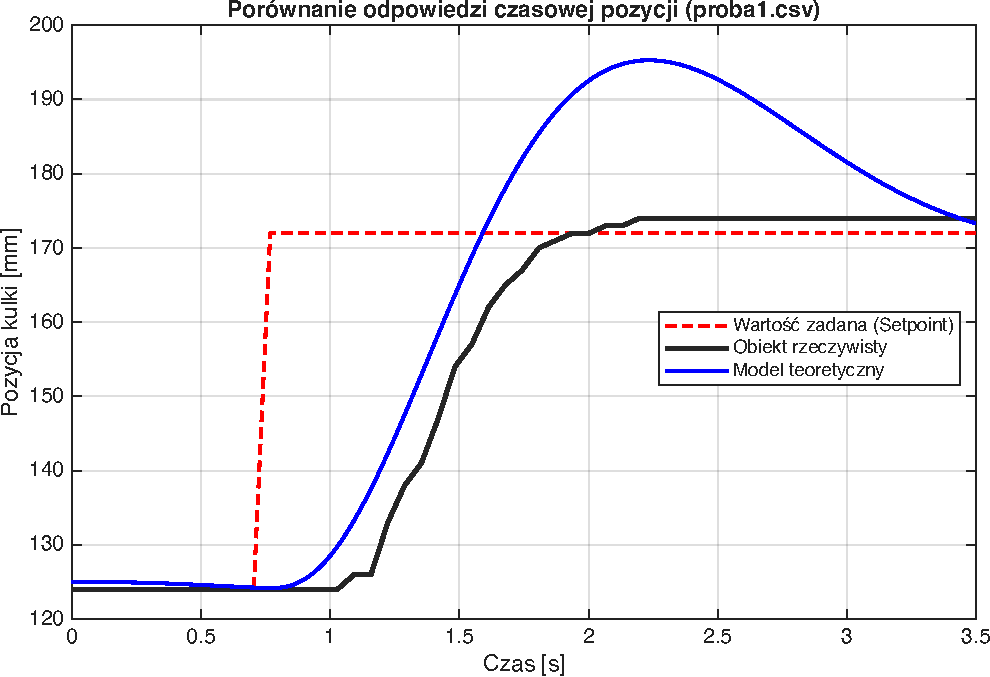
\includegraphics[width=0.9\linewidth]{4-wyniki-eksperymentalne/img/odpowiedz_proba1_teoretyczny.pdf}
    \caption{Porównanie odpowiedzi czasowej pozycji kulki z modelem teoretycznym dla skoku w górę (amplituda +48~mm, plik \texttt{proba1.csv})}
    \label{fig:proba1_pos_teor}
\end{figure}

\begin{figure}[H]
    \centering
    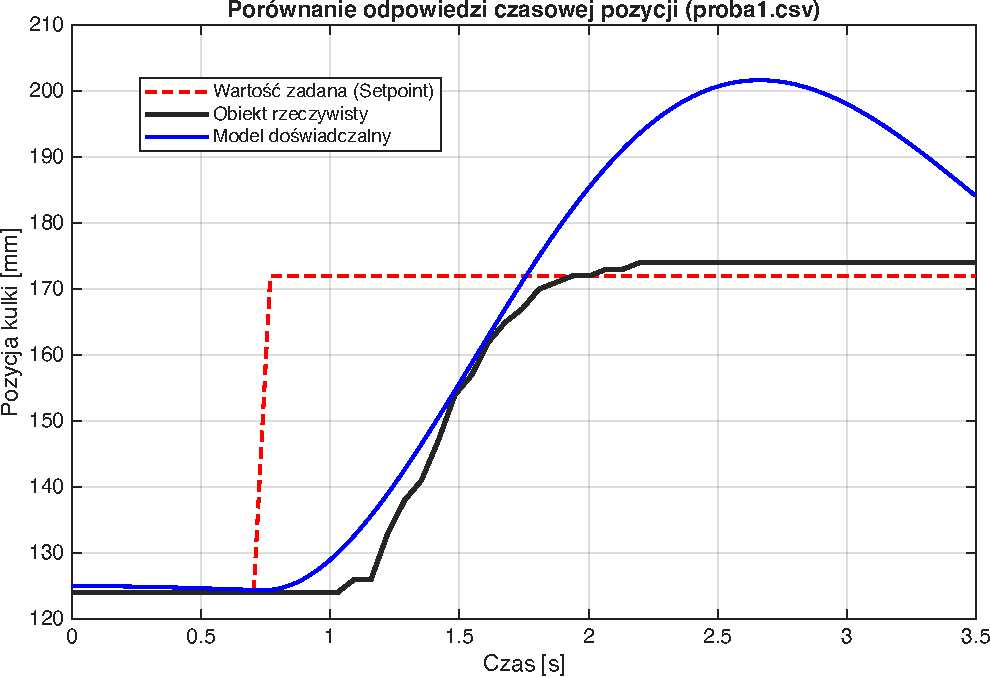
\includegraphics[width=0.9\linewidth]{4-wyniki-eksperymentalne/img/odpowiedz_proba1_doswiadczalny.pdf}
    \caption{Porównanie odpowiedzi czasowej pozycji kulki z modelem doświadczalnym dla skoku w górę (amplituda +48~mm, plik \texttt{proba1.csv})}
    \label{fig:proba1_pos_dosw}
\end{figure}

\begin{figure}[H]
    \centering
    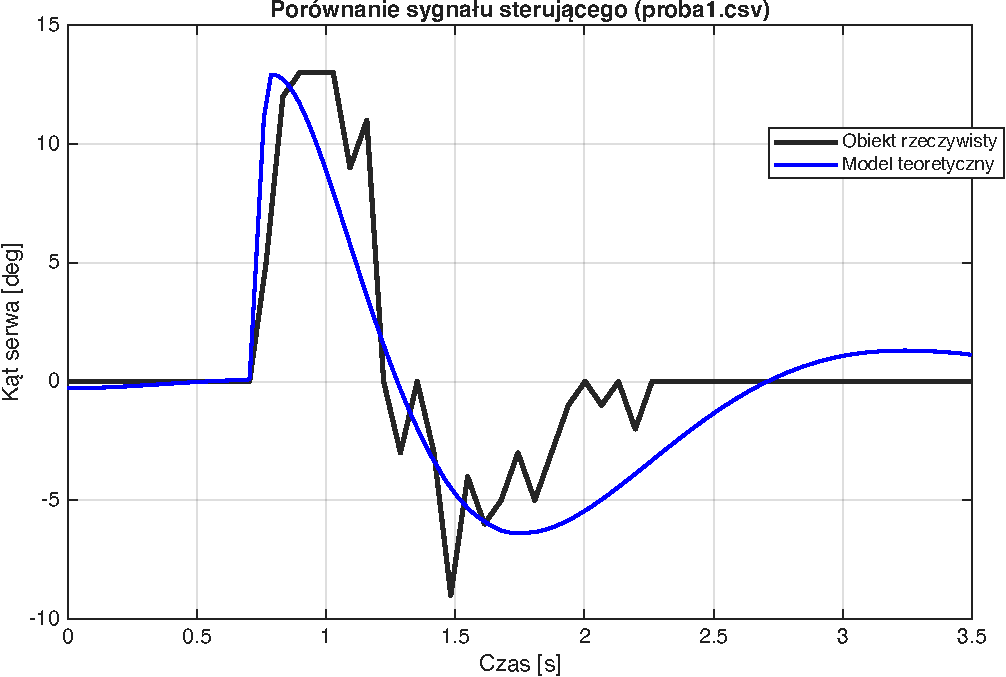
\includegraphics[width=0.9\linewidth]{4-wyniki-eksperymentalne/img/sterowanie_proba1_teoretyczny.pdf}
    \caption{Porównanie sygnału sterującego z modelem teoretycznym dla skoku w górę (amplituda +48~mm, plik \texttt{proba1.csv})}
    \label{fig:proba1_u_teor}
\end{figure}

\begin{figure}[H]
    \centering
    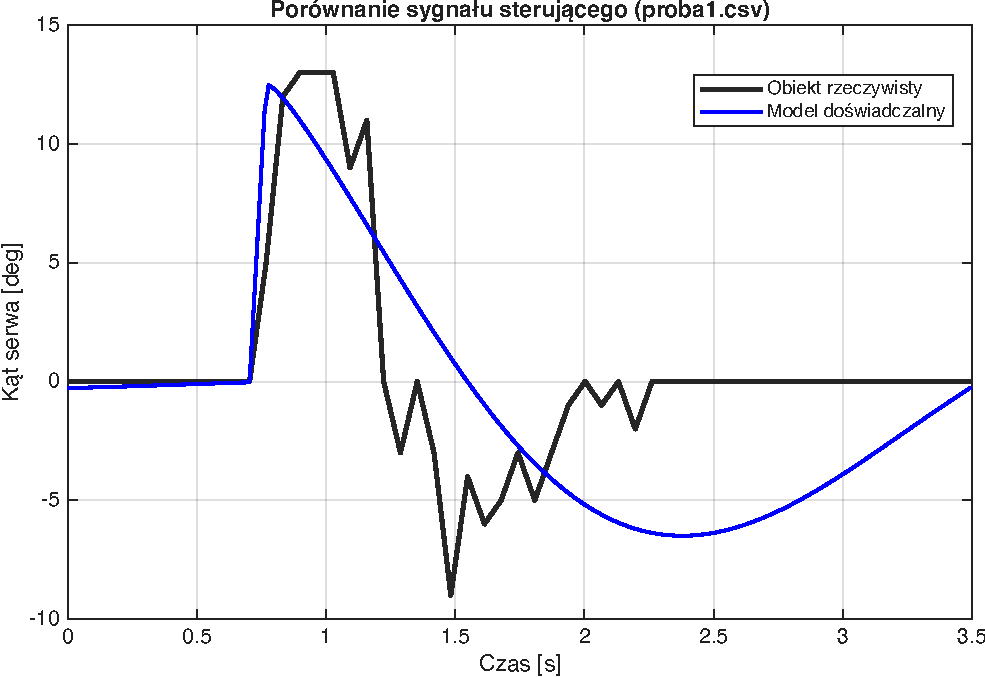
\includegraphics[width=0.9\linewidth]{4-wyniki-eksperymentalne/img/sterowanie_proba1_doswiadczalny.pdf}
    \caption{Porównanie sygnału sterującego z modelem doświadczalnym dla skoku w górę (amplituda +48~mm, plik \texttt{proba1.csv})}
    \label{fig:proba1_u_dosw}
\end{figure}

\begin{figure}[H]
    \centering
    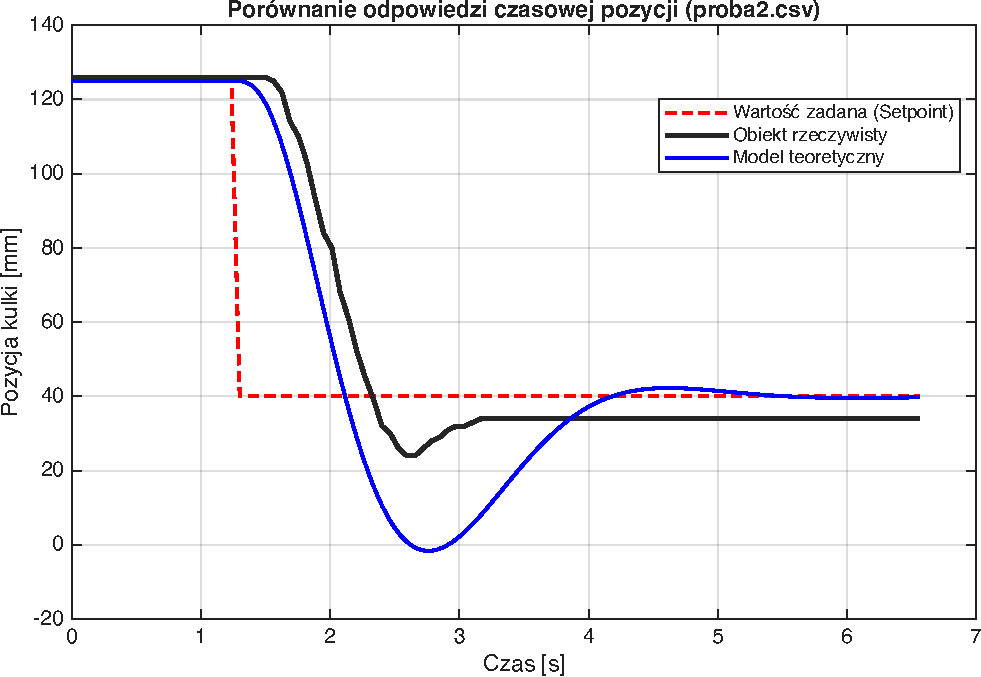
\includegraphics[width=0.9\linewidth]{4-wyniki-eksperymentalne/img/odpowiedz_proba2_teoretyczny.pdf}
    \caption{Porównanie odpowiedzi czasowej pozycji kulki z modelem teoretycznym dla skoku w dół (amplituda -85~mm, plik \texttt{proba2.csv})}
    \label{fig:proba2_pos_teor}
\end{figure}

\begin{figure}[H]
    \centering
    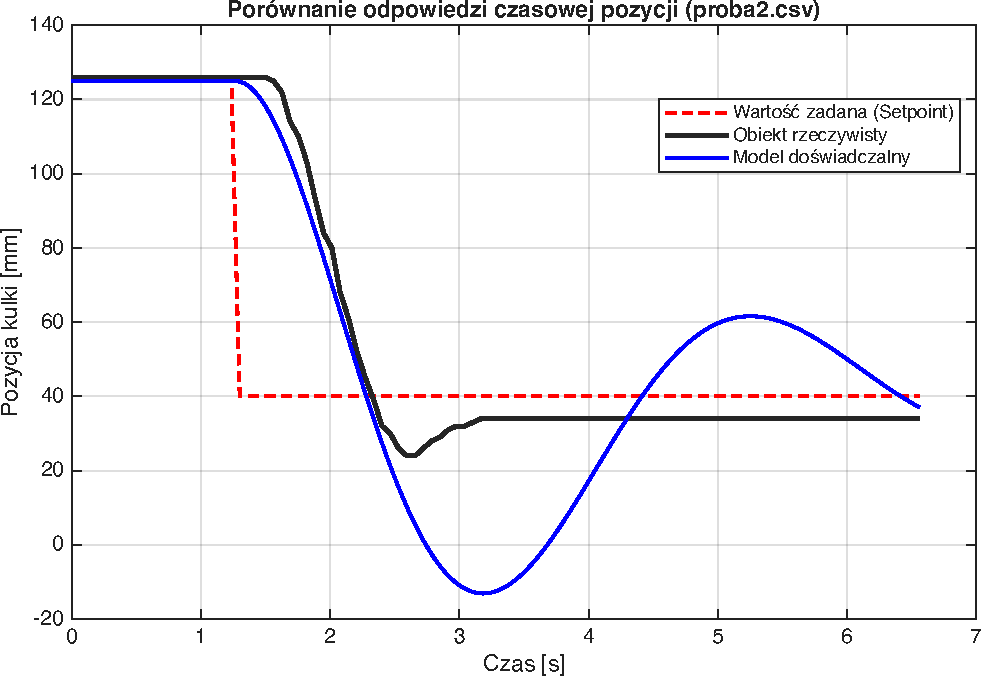
\includegraphics[width=0.9\linewidth]{4-wyniki-eksperymentalne/img/odpowiedz_proba2_doswiadczalny.pdf}
    \caption{Porównanie odpowiedzi czasowej pozycji kulki z modelem doświadczalnym dla skoku w dół (amplituda -85~mm, plik \texttt{proba2.csv})}
    \label{fig:proba2_pos_dosw}
\end{figure}

\begin{figure}[H]
    \centering
    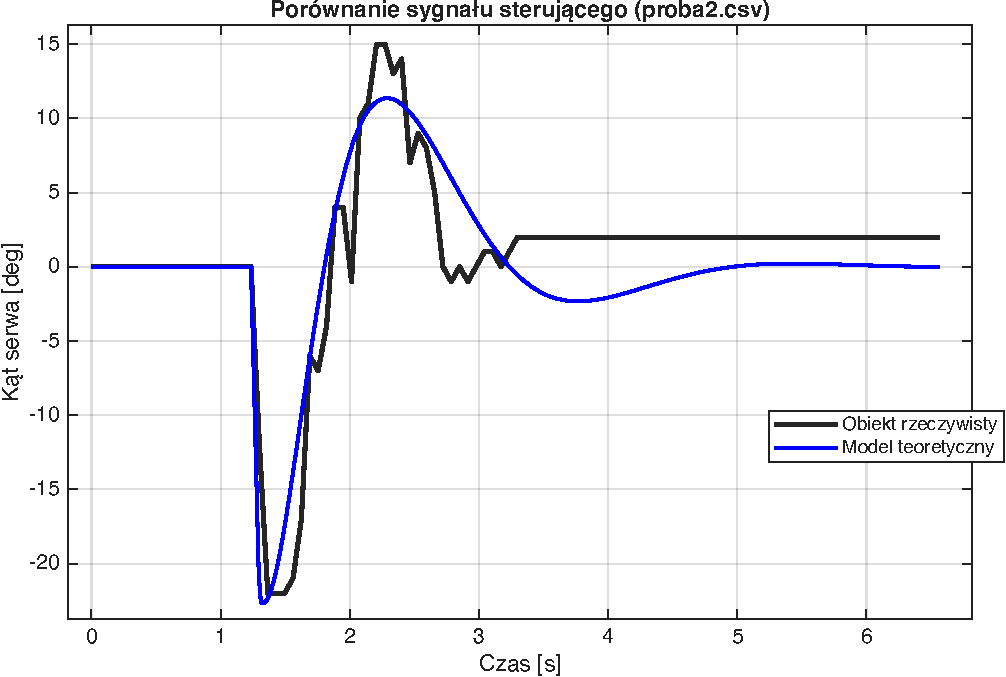
\includegraphics[width=0.9\linewidth]{4-wyniki-eksperymentalne/img/sterowanie_proba2_teoretyczny.pdf}
    \caption{Porównanie sygnału sterującego z modelem teoretycznym dla skoku w dół (amplituda -85~mm, plik \texttt{proba2.csv})}
    \label{fig:proba2_u_teor}
\end{figure}

\begin{figure}[H]
    \centering
    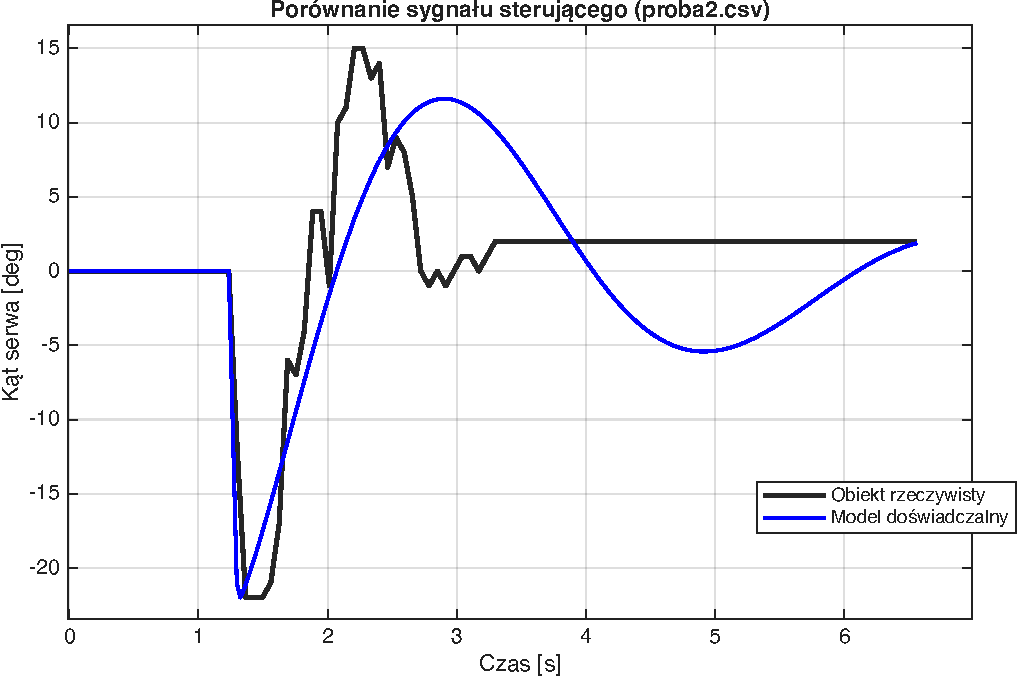
\includegraphics[width=0.9\linewidth]{4-wyniki-eksperymentalne/img/sterowanie_proba2_doswiadczalny.pdf}
    \caption{Porównanie sygnału sterującego z modelem doświadczalnym dla skoku w dół (amplituda -85~mm, plik \texttt{proba2.csv})}
    \label{fig:proba2_u_dosw}
\end{figure}

\section{Analiza ilościowa wskaźników jakości}
\label{sec:wskazniki}

Porównania ilościowego dokonano na podstawie czterech kryteriów:
przeregulowania ($\kappa$), czasu regulacji ($t_s$) dla tunelu tolerancji
$\pm 5\%$, wskaźnika całkowego ITAE oraz kosztu sterowania ($J_u$).
Zestawienie wskaźników dla skoków przedstawiono w tabeli~\ref{tab:wskazniki}.

\begin{table}[H]
\centering
\caption{Zestawienie wskaźników jakości regulacji}
\label{tab:wskazniki}
\small
\setlength{\tabcolsep}{4pt}
\begin{tabular}{lcccc}
\toprule
\textbf{Próba / Obiekt} & \textbf{$\kappa$ [\%]} &
\textbf{Czas reg. $t_s$ [s]} & \textbf{ITAE [mm$\cdot\text{s}^2$]} &
\textbf{$J_u$ [$\text{deg}^2\cdot\text{s}$]} \\ \midrule
\textbf{Próba 1 (Skok +48 mm)} \\
- Obiekt rzeczywisty & 4.17 \% & 0.98 s & 17.64 & 70.07 \\
- Model teoretyczny  & 48.53 \% & 2.62 s & 49.49 & 61.04 \\
- Model doświadczalny & 61.83 \% & >2.73 s & 81.42 & 82.07 \\ \midrule
\textbf{Próba 2 (Skok -85 mm)} \\
- Obiekt rzeczywisty & 18.82 \% & > 5.26 s & 106.81 & 245.21 \\
- Model teoretyczny  & 48.98 \% & 2.60 s & 95.83 & 194.54 \\
- Model doświadczalny & 62.49\% & 4.86 s & 265.02 & 281.11 \\ \bottomrule
\end{tabular}
\end{table}

\section{Analiza i omówienie wyników}
\label{sec:omowienie}

\subsection{Zbieżność sygnału sterującego i przyczyny rozbieżności}
Wykresy sygnału sterującego z symulacji oraz obiektu rzeczywistego (rysunki
\ref{fig:proba1_u_teor}, \ref{fig:proba1_u_dosw}, \ref{fig:proba2_u_teor} oraz
\ref{fig:proba2_u_dosw}) wykazują zgodność pod względem amplitudy początkowej.
Charakterystyczne pierwsze wychylenie (pik sterowania) osiąga na obiekcie
rzeczywistym oraz w modelach podobne wartości (ok. $+13^{\circ}$ do $-9^{\circ}$
dla skoku w górę oraz $+15^{\circ}$ do $-22^{\circ}$ dla skoku w dół). Ponieważ
człon różniczkujący w kodzie STM32 oraz w modelach Simulink jest zaimplementowany
w konfiguracji \textit{Derivative-on-Measurement} (działa bezpośrednio na pomiar
pozycji kulki, a nie na uchyb), nie reaguje on na nagły skok wartości zadanej.
Wobec tego początkowy pik sterowania wynika wyłącznie z działania członu
proporcjonalnego ($P = K_p \cdot e$). W próbie pierwszej, przy uchybie początkowym
$e = 48$~mm, teoretyczna wartość członu P wynosi $0.26 \cdot 48 \approx 12.48^{\circ}$,
co idealnie pokrywa się z zarejestrowanym pikiem sterowania. Fakt ten stanowi
praktyczne potwierdzenie poprawności przeliczenia wzmocnień regulatora oraz
wiarygodności wzmocnienia samego modelu w początkowej fazie ruchu.

Po początkowym piku sygnału sterujacego mozna zaobserwować silne rozbieności miedzy rzeczywistym obiketem i modelami. Na
rzeczywistym obiekcie, dzięki obecności silnego tarcia, pozycja kulki szybko się
ustala bez znaczącego przeregulowania, co powoduje spadek uchybu i powrót sygnału
sterowania do okolic zera. W modelach Simulink, pozbawionych oporów ruchu, kulka
wpada w silne oscylacje wokół wartości zadanej. W efekcie regulator w symulacji próbuje
przeciwdziałać tym wahaniom, co generuje sinusoidalne oscylacje sygnału
sterującego, całkowicie rozbieżne w fazie i amplitudzie z sygnałem rzeczywistym.

\subsection{Wpływ fizycznych oporów ruchu i tarcia}
Rzeczywisty przebieg pozycji kulki (rysunki \ref{fig:proba1_pos_teor},
\ref{fig:proba1_pos_dosw}, \ref{fig:proba2_pos_teor} oraz
\ref{fig:proba2_pos_dosw}) wykazuje znacznie silniejsze tłumienie (bardzo małe
przeregulowanie: $\kappa = 4.17\%$ dla skoku w górę oraz $\kappa = 18.82\%$ dla
skoku w dół) w porównaniu do symulacji. Wynika to z faktu, że
liniowy model matematyczny obiektu $\frac{K}{s^2}$ opisuje idealny, beztarciowy
ruch toczny kulki po płaskiej powierzchni. W rzeczywistym układzie na kulkę
działają opory toczenia, tarcie w łożyskach oraz opór powietrza. Te zjawiska
działają jak naturalne sprzężenie zwrotne od prędkości (tłumienie wiskotyczne
$b\cdot\dot{x}$), które pochłania energię kinetyczną kulki, tłumi drgania
i drastycznie skraca rzeczywisty czas regulacji (do $0.98$~s w próbie 1).

\subsection{Paradoks tłumienia modelu bez oporów ruchu}
Interesującym zjawiskiem zaobserwowanym w badaniach symulacyjnych jest fakt,
że model doświadczalny (o mniejszym wzmocnieniu $K=11.93$) charakteryzuje się
większym przeregulowaniem ($\kappa \approx 62\%$) i dłuższym czasem regulacji
(lub wręcz brakiem ustalenia w czasie symulacji, jak w rysunkach
\ref{fig:proba1_pos_dosw} i \ref{fig:proba2_pos_dosw}) niż model teoretyczny
($K=20.55$, gdzie $\kappa \approx 48\%$). Zjawisko to wynika bezpośrednio
z teorii sterowania układów drugiego rzędu. Współczynnik tłumienia $\zeta$
układu zamkniętego z regulatorem PD (przy pominięciu członu I oraz stałej
czasowej serwa) można wyrazić uproszczonym wzorem:
\begin{equation}
    \zeta = \frac{K_d}{2} \sqrt{\frac{K}{K_p}}
\end{equation}
Pominięcie członu całkującego w powyższej analizie jest w pełni uzasadnione
teoretycznie, ponieważ jego wzmocnienie ($K_i = 0.2$) jest relatywnie małe
w stosunku do dynamiki całego układu. Wpływ całki na dominującą parę biegunów
zespolonych układu trzeciego rzędu (którym staje się układ po dodaniu członu I)
jest znikomy, a dynamika drgań pozostaje zdominowana przez te dwa bieguny.
W modelu pozbawionym naturalnego tarcia ($b=0$), jedynym źródłem tłumienia jest
człon różniczkujący $K_d$. Ponieważ wzmocnienie obiektu $K$ znajduje się
w liczniku pod pierwiastkiem, zmniejszenie wzmocnienia obiektu z $20.55$ do
$11.93$ (w modelu doświadczalnym) powoduje spadek współczynnika tłumienia
$\zeta$, co objawia się silniejszymi i dłużej trwającymi oscylacjami.

\subsection{Tarcie statyczne i uchyb ustalony}
Rzeczywisty obiekt wykazuje opóźnienie w rozpoczęciu ruchu (wynoszące ok.
$0.23$~s od momentu skoku wartości zadanej). Wynika to z obecności tarcia
statycznego, które całkowicie blokuje ruch kulki do momentu, w którym
belka pochyli się pod odpowiednim kątem, generując składową siły grawitacji
zdolną pokonać opór początkowy. Ponieważ idealne modele w Simulinku nie zawierają
nieliniowości tarcia statycznego ani luzu przekładni, symulowany ruch kulki
zaczyna się natychmiast po zmianie setpointu ($t = t_{step}$), co stanowi główną
różnicę w początkowej fazie odpowiedzi.

Tarcie statyczne oraz luz mechaniczny na przekładni serwomechanizmu
są również odpowiedzialne za powstanie uchybu ustalonego (w próbie 1 kulka
zatrzymała się na pozycji $174$~mm zamiast zadanych $172$~mm, a w próbie 2 na
$46$~mm zamiast $40$~mm). Gdy uchyb jest niewielki (rzędu 2--6 mm), generowane
przez regulator pochylenie belki (ok. $1^{\circ}$--$2^{\circ}$) jest zbyt małe,
aby pokonać próg tarcia statycznego, przez co kulka zatrzymuje się przed
osiągnięciem dokładnego punktu docelowego.

\subsection{Szumy pomiarowe, filtracja i szpilki sterowania}
W rzeczywistym sygnale sterującym z STM32 widoczne są liczne zakłócenia o wysokiej
częstotliwości (tzw. szpilki). W kodzie mikrokontrolera
zaimplementowano filtrację różniczki za pomocą algorytmu wykładniczego średniej
kroczącej (EMA) ze współczynnikiem $\alpha = 0.5$ oraz strefę nieczułości
(\texttt{D\_DEADBAND = 0.1} mm). Pomimo tych zabezpieczeń, w sygnale sterującym
wciąż występują szpilki.

Wynika to ze specyfiki dyskretyzacji pozycji w systemie wizyjnym, który zaokrągla
pomiar do pełnych milimetrów. Każdy pojedynczy przeskok pozycji kulki o 1 mm
jest traktowany jako nagła zmiana, która z łatwością przekracza strefę nieczułości.
Przy współczynniku $\alpha = 0.5$ filtr tłumi zakłócenie jedynie o połowę, co przy
wysokim wzmocnieniu różniczkującym $K_d = 4.4$ przekłada się na nagłą zmianę
sygnału sterującego o $4.4 \cdot 0.5 = 2.2^{\circ}$. Te powtarzające się impulsy
są bezpośrednią przyczyną szumów sterowania. W celu dalszego wygładzenia sygnału,
możliwe byłoby zwiększenie siły filtrowania (zmniejszenie wartości $\alpha$) lub
zastosowanie bardziej zaawansowanych algorytmów estymacji, takich jak filtr
Kalmana pracujący bezpośrednio na sygnale pozycji.

\subsection{Wnioski końcowe i ocena dokładności modeli}
Dokonując ostatecznego porównania modeli, należy przeanalizować ich zachowanie w układzie
zamkniętym w odniesieniu do obiektu rzeczywistego. Dane z tabeli~\ref{tab:wskazniki}
wskazują, że model teoretyczny charakteryzuje się mniejszym przeregulowaniem (ok.
$48\%$--$49\%$) i niższym wskaźnikiem ITAE niż model doświadczalny (przeregulowanie
ok. $62\%$). W beztarciowym środowisku symulacyjnym to model teoretyczny wydaje się być
zatem bliższy rzeczywistemu zachowaniu obiektu (który wykazuje bardzo silne tłumienie).

Stanowi to jednak opisany wcześniej paradoks matematyczny wynikający ze struktury
wzoru na tłumienie $\zeta = \frac{K_d}{2}\sqrt{\frac{K}{K_p}}$. Wyższe wzmocnienie
teoretyczne ($K_{\text{teor}} = 20.55$) sztucznie zwiększa tłumienie różniczkujące w symulacji,
maskując brak fizycznego tarcia w modelu. 

Z fizycznego punktu widzenia to model doświadczalny ($K_{\text{dosw}} = 11.93$) jest
bardziej adekwatny. Różnica we wzmocnieniach wynika z faktu, że podczas identyfikacji
doświadczalnej (metodą odpowiedzi skokowej w układzie otwartym) wyznaczono wzmocnienie
skumulowane. Zjawiska takie jak poślizg kulki, mechanika drutu łączącego serwo z belką, 
a przede wszystkim dynamika samego serwomechanizmu
(która w identyfikacji doświadczalnej została uproszczona i włączona bezpośrednio
we wzmocnienie statyczne obiektu) powodują efektywne zmniejszenie dynamiki ruchu kulki.
W przypadku rozbudowy modelu o nieliniowy człon tarcia rzeczywistego, model doświadczalny
zapewniłby prawdopodobnie wyższą dokładność odwzorowania obiektu, podczas gdy model teoretyczny
wykazywałby przesterowanie.
